\documentclass{article}
\usepackage{graphicx}
\graphicspath{ {images/} }

\title{ProblemSet 6}
\author{Yue Wu}
\date{March 2018}



\begin{document}

\maketitle

\section{Clean Data}

Clean data

1. Some games don't have developer. I replace 'NA' by 'None'.

2. Through the study of data, I consider the missing values are random. Because there is no relationship between the missing value and other observations. So I drop observations which have missing values.

3. Due to some observations are highly skewed, I use log and scale to transform them.
I use 'boxplot' and 'hist' commands to check all observations, there are many outliers and their shapes looks skewed.
To make the plot looks normal likely, I use 'log' and 'scale' to transform those observations into new vectors.  


\section{Visualizations}

Visualizations

The plot below shows the frequency of different type of games. From this graph we can see that what type of games are game producers would like to make.

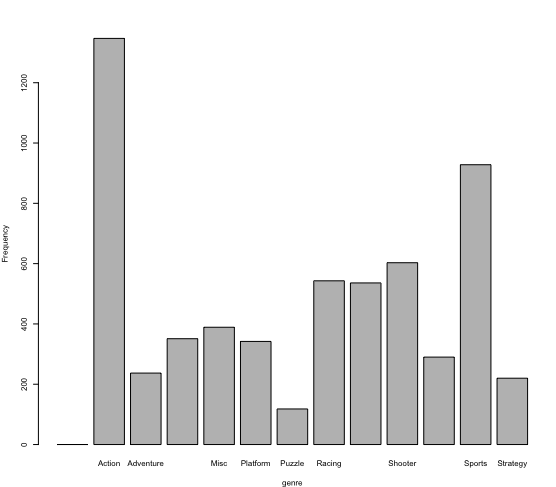
\includegraphics[scale=0.5]{PS6a_wu.png}


The plot below shows the.relationship.between type of game and global sales.From this graph, we can see that what type of games are players would like to buy.


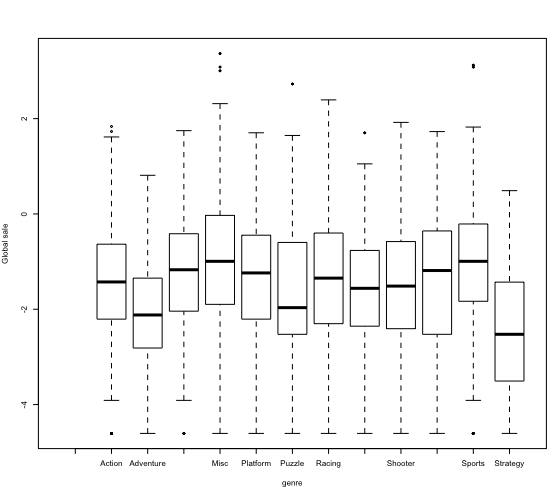
\includegraphics[scale=0.5]{PS6b_wu.png}


The plot below show the relationship between critic score and global sales. Through the graph, we can see that they have positive relationship. So critic score has positive affect on global sales.


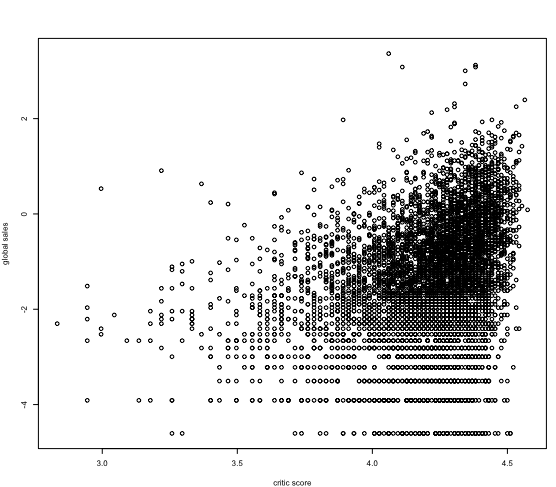
\includegraphics[scale=0.5]{PS6c_wu.png}

